\section{What the Selected Evidence Supports}
Figure~\ref{fig:evidence} maps the selected reports by publication status, environment, action, and endpoint. It is categorical: neither rows nor colors define a performance ranking. The central pattern is a progression from answers and dialogue toward verifiable benchmark effects, with persistent separation between simulation and live patient care.

\begin{figure*}[t]\centering
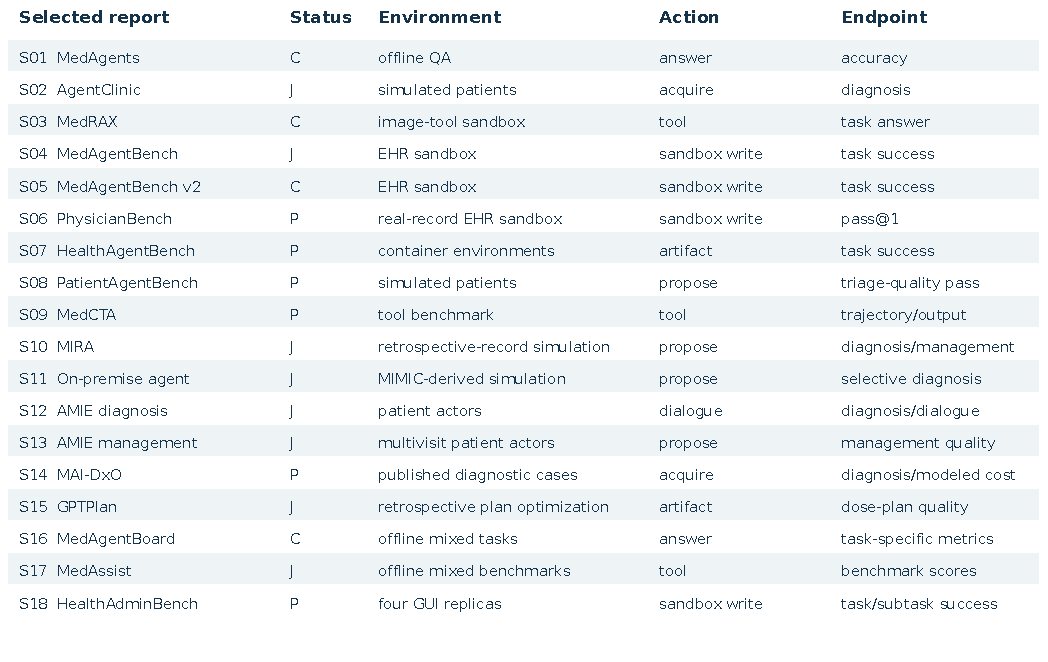
\includegraphics[width=\textwidth]{figures/fig2_evidence_map.pdf}
\caption{Purposive evidence map of 18 empirical reports. J: journal; C: conference; P: preprint. Environments and endpoints are recorded under the cited versions. These categories do not measure prevalence, quality scores, or clinical readiness.}\label{fig:evidence}
\end{figure*}

\subsection{Reasoning and diagnostic interaction}
MedAgents studies collaborative medical reasoning on question-answering tasks \cite{medagents2024}. It is useful as a boundary comparator because an improved answer does not verify a clinical action. AgentClinic introduces interactive simulated patient evaluation \cite{agentclinic2026}, moving the assessment toward information acquisition. MedRAX combines medical imaging tools with an agent workflow \cite{medrax2025}; success remains attached to benchmark queries rather than prospective radiology decisions.

AMIE evaluates diagnostic consultation with patient actors \cite{amie2025}. Its management extension investigates multivisit, guideline-grounded interaction \cite{amiemanagement2026}. These designs provide richer assessments of dialogue and recommendations than static examination questions. Actors, however, are not patients receiving autonomous treatment. Neither a conversational recommendation nor an actor-based outcome verifies that a medication order was admissible, committed correctly, and followed safely. MAI-DxO evaluates sequential information gathering on 304 published diagnostic cases and models testing cost \cite{maid2025}. Modeled test cost must not be interpreted as measured expenditure or effectiveness in routine care.

\subsection{Execution-grounded EHR and tool tasks}
MedAgentBench evaluates 300 tasks over 100 patient profiles in an EHR sandbox \cite{medagentbench2025}. Its second version reports different conditions on original and new tasks \cite{medagentbenchv2}. The memory-related results and newly constructed tasks require separate interpretation; combining them would obscure both feedback exposure and distribution shift.

PhysicianBench uses real-record EHR tasks with script-verified checkpoints \cite{physicianbench2026}. Its 100 long-horizon tasks involve 670 checkpoints and an average of 27 calls. The best reported pass@1 is 46\%. This is stronger evidence of execution difficulty than a static QA score, but still evidence from a benchmark environment. The title's ``real-world'' wording describes grounding and workflow realism; it should not be converted into a prospective deployment claim.

HealthAgentBench spans 54 tasks in seven categories with distinct environments and executable artifacts \cite{healthagentbench2026}. PatientAgentBench studies simulated patient interaction and triage \cite{patientagentbench2026}. MedCTA evaluates tool-use trajectories as well as outputs \cite{medcta2026}. Together these reports make task completion, intermediate decisions, and evaluation definitions more visible. Their scores remain conditional on supplied environments and adjudication methods.

\begin{table*}[t]\caption{Selected quantitative anchors: preserve endpoint and context}\label{tab:anchors}\centering\footnotesize
\begin{tabularx}{\textwidth}{@{}p{.15\textwidth}p{.35\textwidth}Y@{}}\toprule
Report & Reported anchor & Interpretation boundary \\ \midrule
MedAgentBench v2 \cite{medagentbenchv2} & Original tasks: 91\% without memory, 98\% with feedback memory; new tasks: 266/300 (88.67\%). & Distinct sets/configurations; not a pooled estimate.\\
PhysicianBench \cite{physicianbench2026} & 100 tasks, 670 checkpoints, average 27 calls; best 46\% pass@1. & Real-record sandbox execution; not live clinical utility.\\
HealthAgentBench \cite{healthagentbench2026} & 54 tasks, seven categories; best approximately 42\% task success. & Heterogeneous artifact tasks; no cross-benchmark ranking.\\
PatientAgentBench \cite{patientagentbench2026} & 1,200 scenarios, ten models; triage-quality pass rates 32--88\%. & Model/scenario-dependent triage; no verified downstream effect.\\
MedCTA \cite{medcta2026} & 107 tasks and five tools. & Dataset scale, not clinical efficacy or harm rate.\\
MIRA \cite{mira2026} & More than 500 cases, 11 tools, over 85,000 possible actions. & Retrospective simulation and physician comparisons.\\
On-premise agent \cite{onprem2026} & Consistency threshold 0.90: 49.4\% retained, 98.9\% diagnostic accuracy. & Selective diagnostic endpoint; not unsafe committed-action risk.\\
GPTPlan \cite{gptplan2025} & 12 lung IMRT and five cervical VMAT cases. & Abstract-only plan evaluation; no treatment-delivery claim.\\
HealthAdminBench \cite{healthadmin2026} & 135 tasks, 1,698 points; best task 36.3\%; highest subtask 82.8\%. & Different agent configurations achieve the two maxima.\\ \bottomrule
\end{tabularx}\end{table*}

\subsection{Clinical management, planning, and administration}
MIRA integrates diagnostic and management options in retrospective clinical simulations \cite{mira2026}. Its broad tool/action space and physician comparisons make it relevant to action-centered evaluation, but do not establish prospective autonomous patient care. An on-premise system examines operational governance and diagnostic reliability using MIMIC-derived environments \cite{onprem2026,mimiciv2023}. Selective retention of more consistent diagnoses is an important uncertainty result. It does not demonstrate the same risk for committed orders, omission, or downstream outcomes.

GPTPlan concerns radiotherapy plan optimization \cite{gptplan2025}. A generated treatment plan is an artifact that requires further verification and authorization before delivery. Because access here is abstract-only, no detailed claim about its control architecture is used. MedAgentBoard compares approaches across several offline medical tasks \cite{medagentboard2025}; MedAssist evaluates a general tool-oriented agent configuration \cite{medassist2026}. These mixed-task studies caution against treating multi-agent design as an inherent benefit. Additional medical-agent evaluation work likewise motivates explicit task and interface definitions \cite{medicalagentsbench2026}.

HealthAdminBench provides four GUI replicas for EHR, payer, and document workflows \cite{healthadmin2026}. The contrast between task and subtask rates is especially instructive: the reported best end-to-end task success and highest subtask success come from different configurations. Administrative effects can influence care access, eligibility, and delay. Their consequences require evaluation even when the agent never issues a clinical order.

\subsection{Synthesis across heterogeneous endpoints}
Table~\ref{tab:anchors} preserves units and limitations. Three deductions follow from the selected evidence. First, interaction and execution create additional testable failure modes beyond knowledge recall. Second, realistic records or interfaces improve fidelity without removing the distinction between sandbox and clinical deployment. Third, benchmark completion is a necessary capability measure for some workflows but is not sufficient evidence of patient benefit or admissible autonomy. None of the selected reports, under the extracted evaluation designs, establishes prospective autonomous live patient-care effectiveness. This statement is limited to the selected map and is not an assertion about all systems worldwide.
